\section{系统架构与方法论}
\label{sec:methodology}

\begin{figure*}[!t]
    \centering
    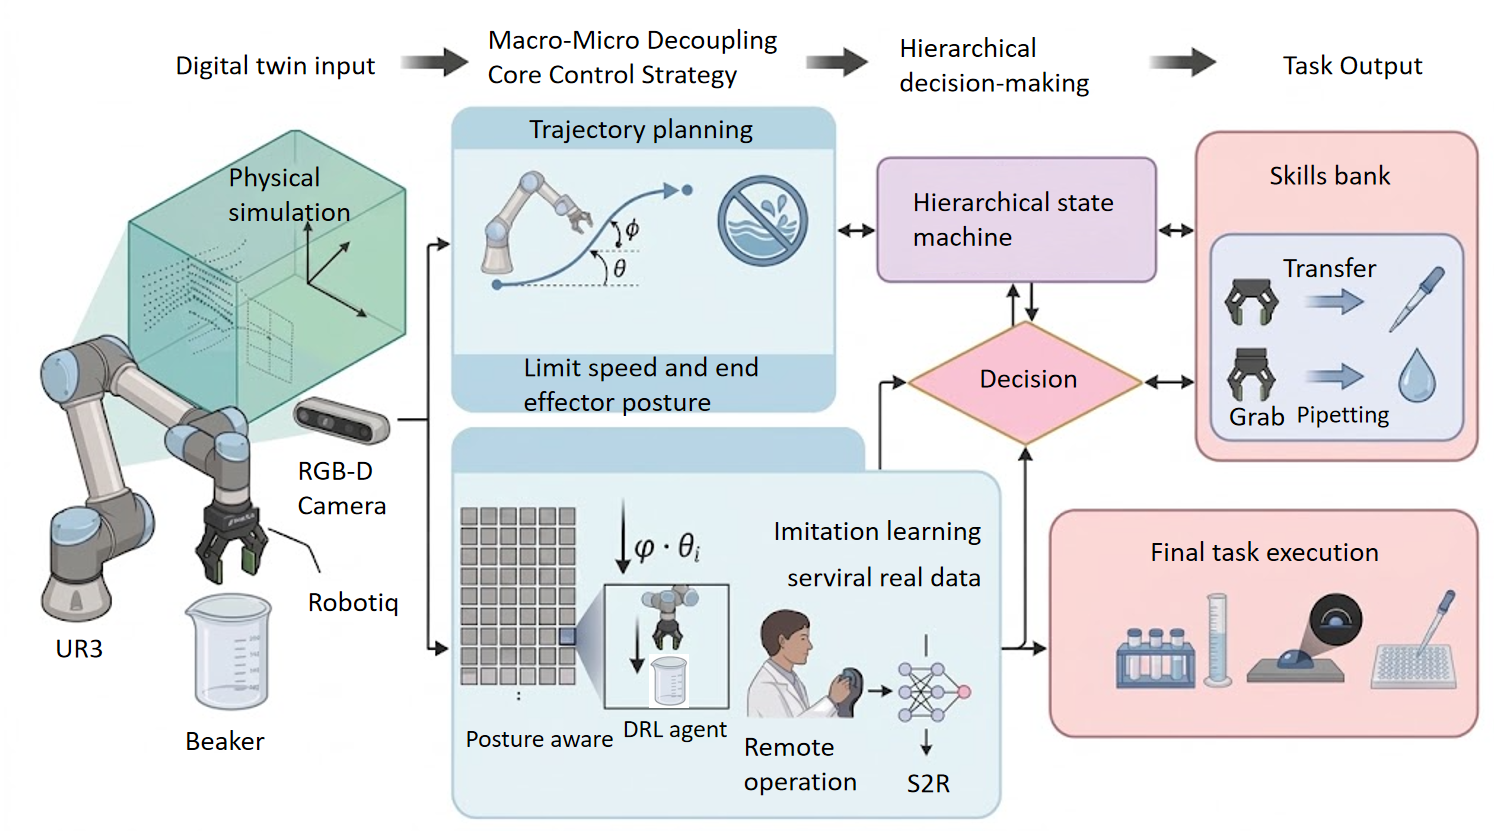
\includegraphics[width=\textwidth]{images/Framework.png}
    \caption{系统控制框架：结合物理仿真与RGB-D感知、约束轨迹规划、姿态感知强化学习、模仿学习与虚实迁移适配，并通过分层状态机调用可复用技能完成实验室任务。}
    \label{fig:overall_framework}
\end{figure*}

本章详细介绍了专为生化自动化化验（包括溶液配置、水滴角检测和梯度稀释）量身定制的多平台混合机器人框架。为了应对异构任务需求，跨工位宏观转移由约束感知经典规划执行，而灵巧的机械臂操作则由融合了大规模并行深度强化学习（DRL）与人在回路模仿学习（IL）的混合学习架构统筹。

\subsection{用于策略训练的仿真环境}
\label{subsec:simulation_training}

图~\ref{fig:simulation_overview}概括了环境构建、技能并行训练及物理部署过程。
\begin{figure*}[!t]
    \centering
    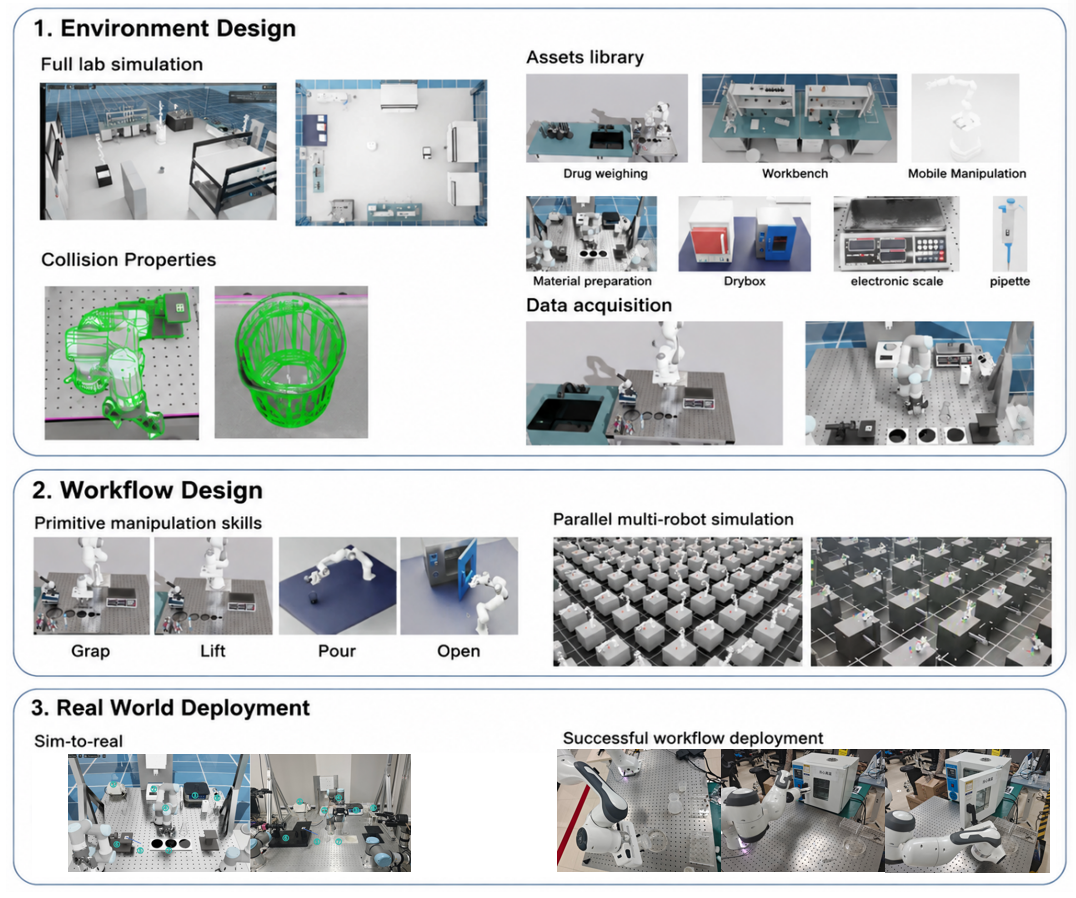
\includegraphics[width=0.94\textwidth]{images/environment_design2.png}
    \caption{仿真开发与物理部署总览：实验室环境与资产构建、碰撞建模和数据采集；操作技能开发与并行仿真；以及实验室操作的虚实迁移部署。}
    \label{fig:simulation_overview}
\end{figure*}

为了实现接触密集型任务的无风险训练与预验证，我们利用NVIDIA Isaac Sim构建了高保真仿真环境。在GPU加速张量物理引擎的驱动下，仿真环境能够准确建模刚体动力学、关节力矩和摩擦接触。夹爪和器材固定架均赋予了有符号距离场（SDF）碰撞网格，以实现无穿透的接触仿真。至关重要的是，独立的Python API架构实现了跨数千个并发虚拟环境的GPU并行化，彻底突破了物理机器人学习中样本效率低下的瓶颈。

\subsection{仿真环境与实体环境的状态同步}
\label{subsec:state_sync}

图~\ref{fig:state_sync_mechanism}展示坐标与时间对齐、观测有效性检查，以及带来源标记的虚拟实验台状态更新。
\begin{figure*}[!t]
    \centering
    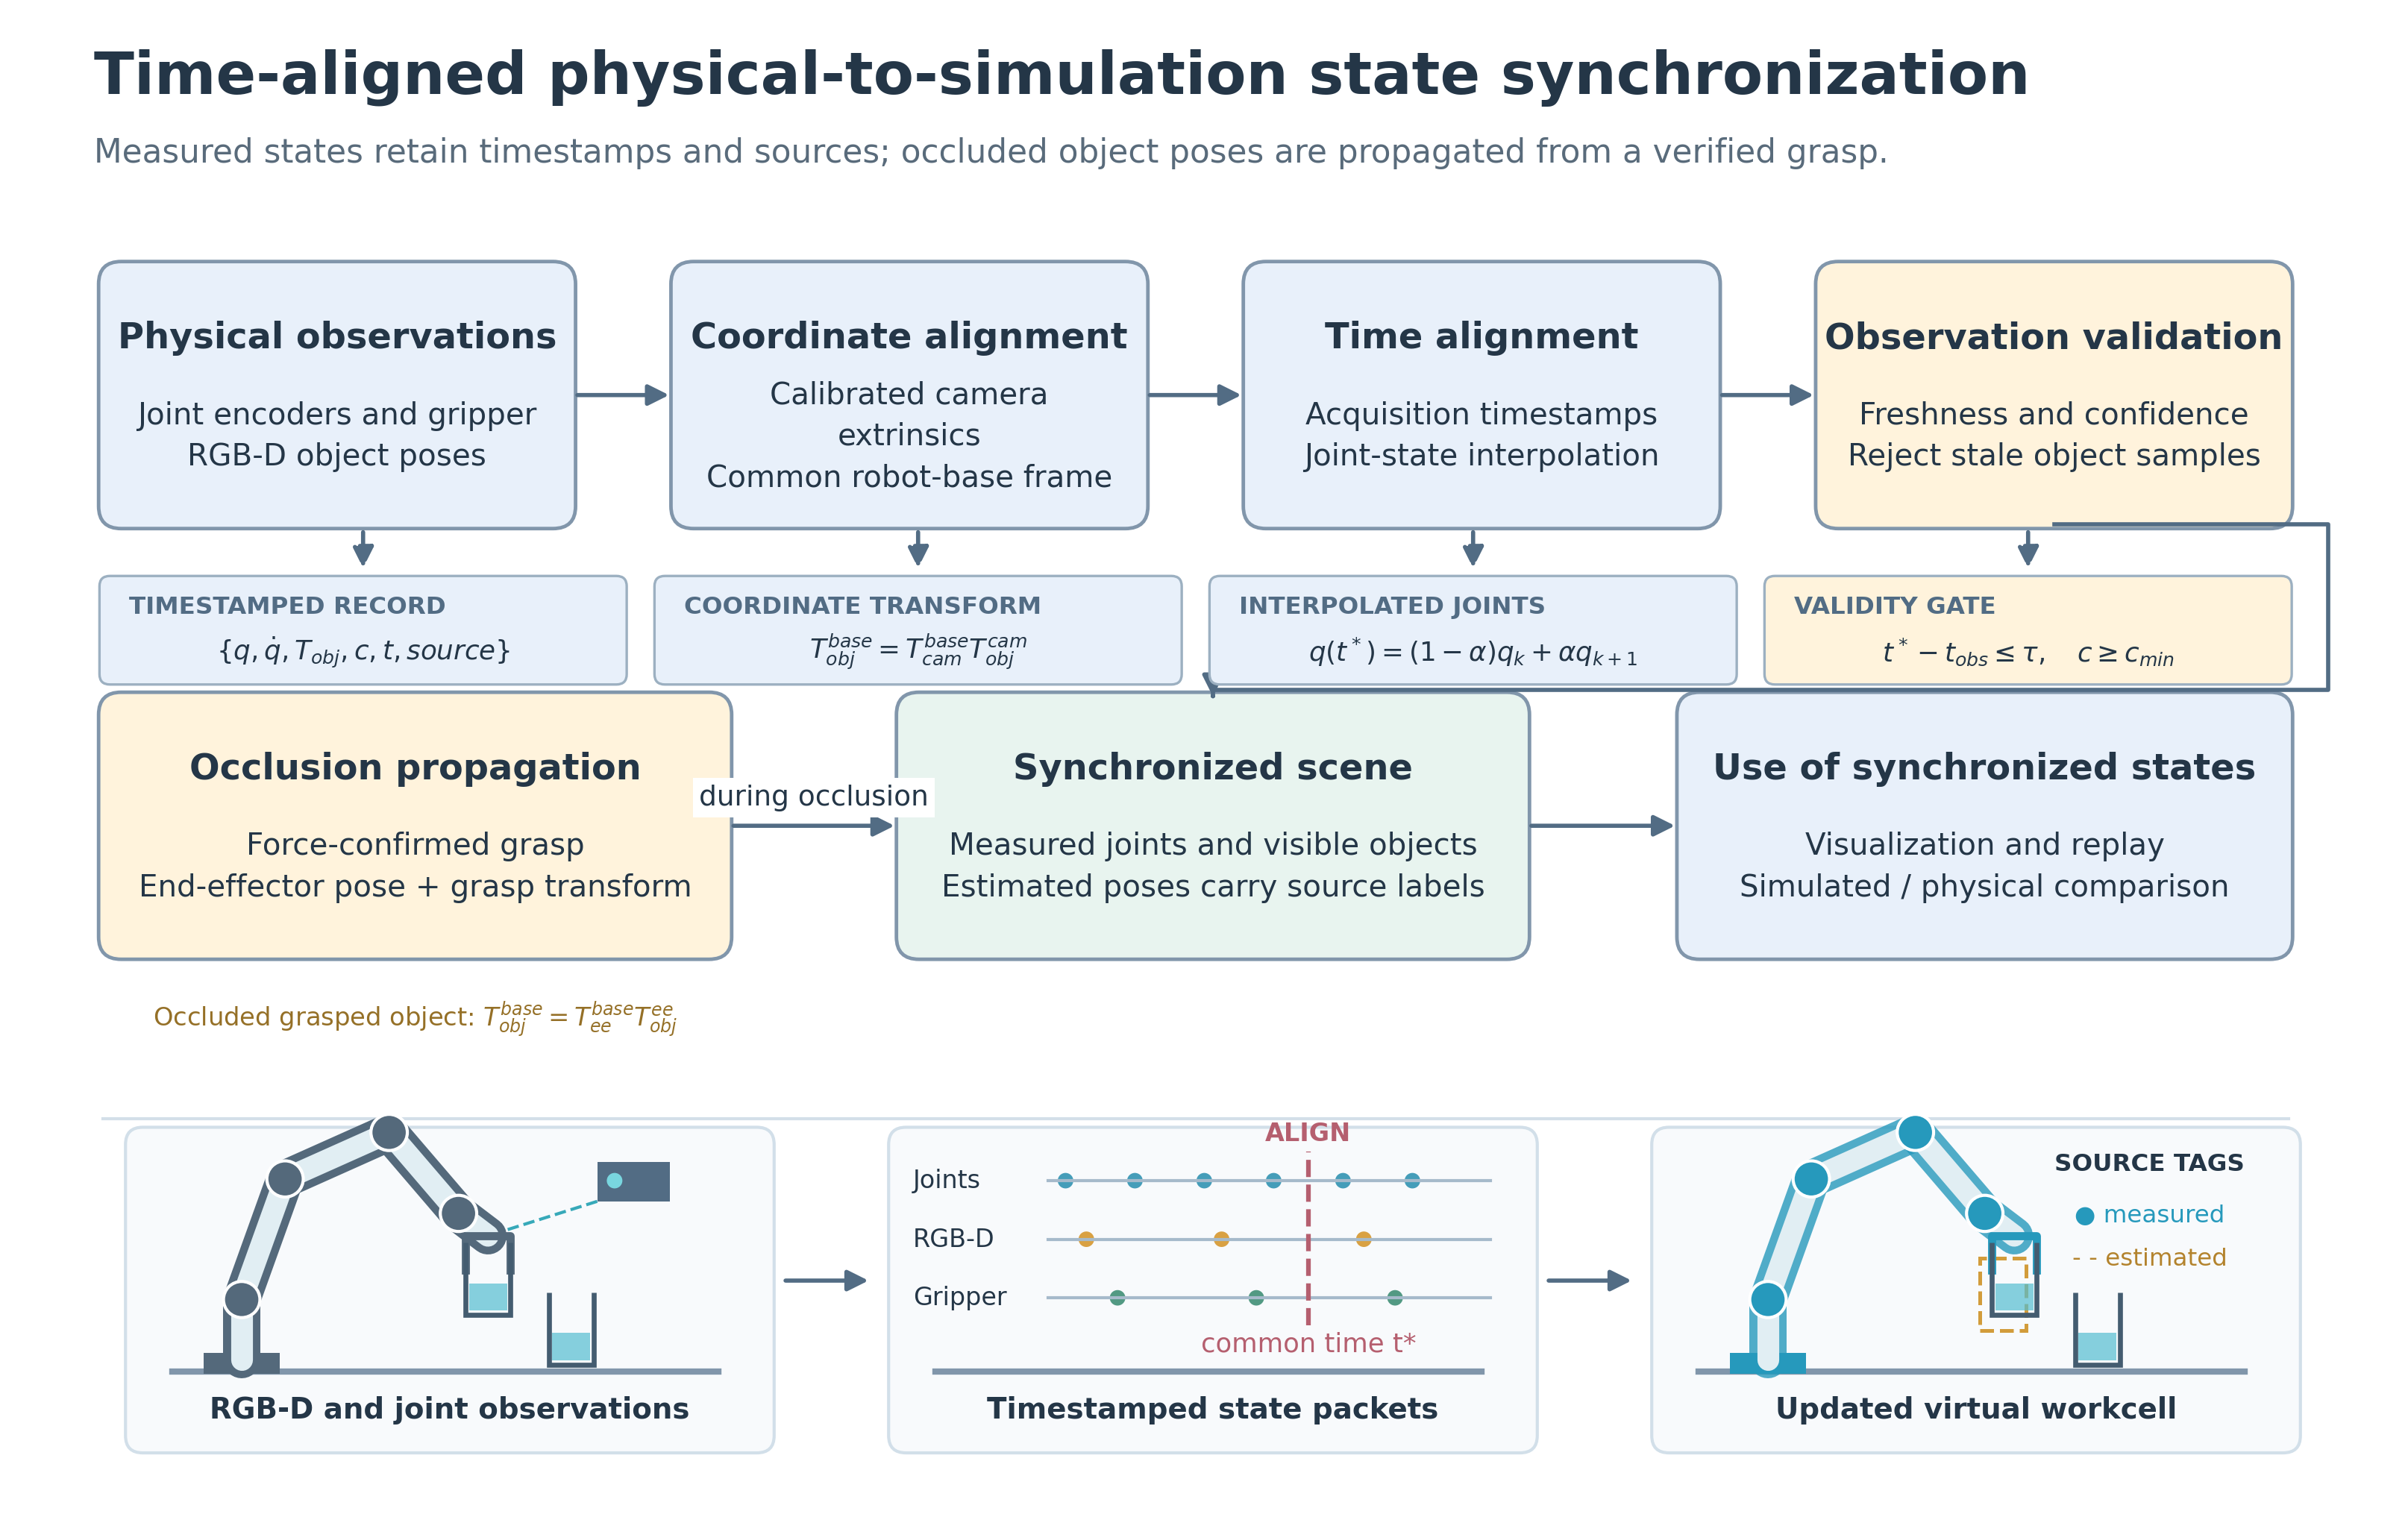
\includegraphics[width=\textwidth]{images/mechanisms/state_synchronization_mechanism.png}
    \caption{时间对齐的实体到仿真状态同步机制。异步关节、RGB-D与夹爪观测对齐到共同时间，并经有效性检查后更新场景。实线与虚线物体轮廓区分测量与传播估计位姿；同步用于可视化和比较，不代表已验证预测闭环控制。机械臂为示意绘制。}
    \label{fig:state_sync_mechanism}
\end{figure*}

我们定义实体机器人与Isaac Sim仿真环境之间的状态接口。关节编码器提供机械臂关节位置$\mathbf q_t$和速度$\dot{\mathbf q}_t$，夹爪提供开合状态与抓取确认信号；RGB-D视觉观测提供可见物体的位置$\mathbf p_{i,t}$、姿态$\mathbf R_{i,t}$及检测置信度。仅在连续观测可靠时估计物体速度。每条状态记录保留采集时间戳和数据来源，以区分直接测量与估计状态。

更新仿真场景前，利用标定外参将视觉观测转换到机器人基座坐标系，并将关节与物体观测对齐到共同时间戳。关节位置在相邻编码器采样之间插值；物体位姿由最近一次有效视觉观测更新。物体在力反馈确认抓取后短暂遮挡时，根据末端位姿和已估计的抓取变换传播其位姿。对过期或低置信度的物体观测不作为当前测量使用。同步后的状态用于可视化和比较仿真与实体轨迹；状态同步本身不能证明仿真预测精度或闭环控制性能。

\subsection{面向宏观导航的约束感知运动规划}
\label{subsec:macro_planning}

% \begin{figure}[htbp]
%     \centering
%     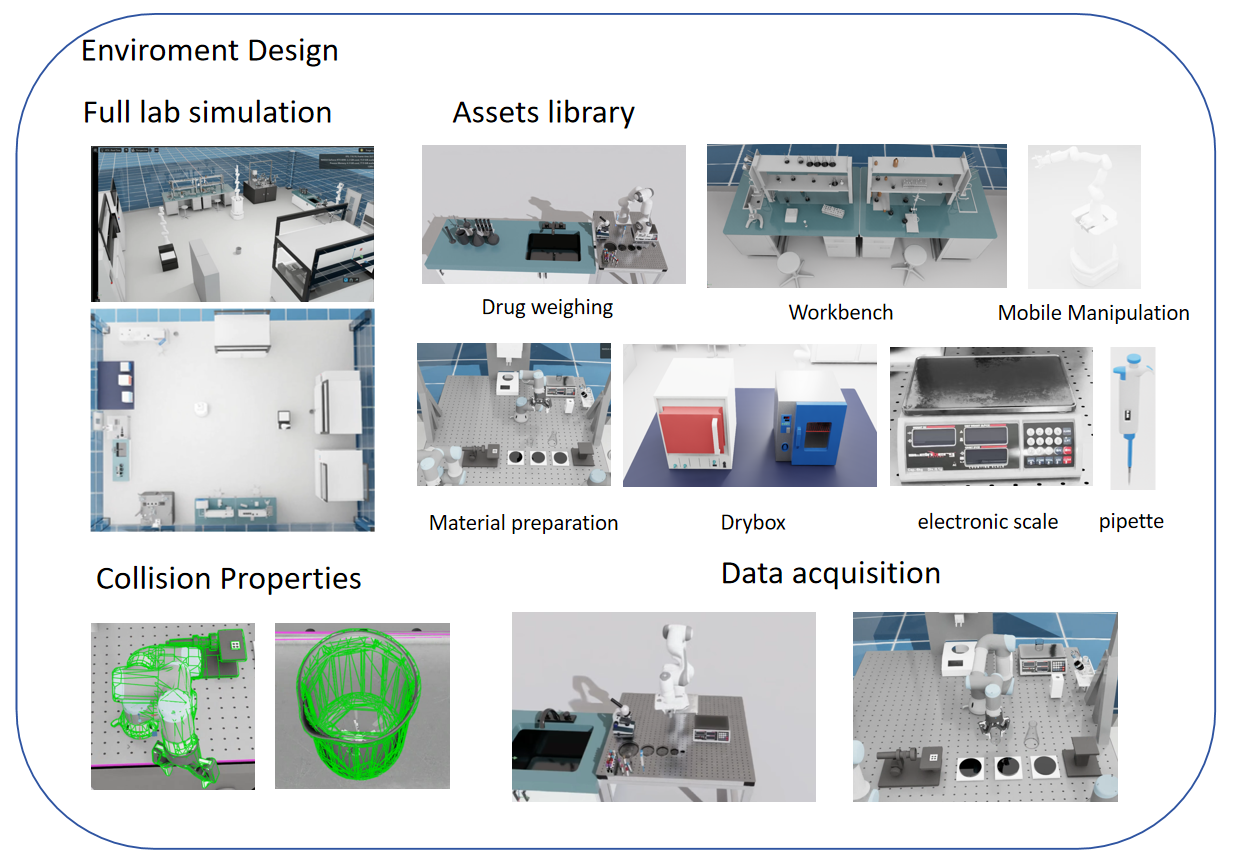
\includegraphics[width=0.9\linewidth]{images/environment_design.png}
%     \caption{基于Isaac Sim构建的高保真仿真环境。该仿真环境集成了UR3机械臂和Robotiq 2F-85平行夹爪，并采用有符号距离场（SDF）碰撞网格实现精确的接触建模。}
%     \label{fig:sim_env}
% \end{figure}

对于工作站之间的宏观转移（例如运送配好的试剂瓶），我们采用约束感知的经典运动规划器。为了防止移动过程中的流体晃动，对末端执行器的横滚角（$\phi$）和俯仰角（$\theta$）施加了严格的任务空间姿态约束：
\begin{equation}
    |\phi(t) - \phi_{\text{target}}| \leq \epsilon_{\phi}, \quad |\theta(t) - \theta_{\text{target}}| \leq \epsilon_{\theta}, \quad \forall t \in [0, T]
\end{equation}
路径平滑被公式化为最小冲击（minimum-jerk）轨迹优化问题：
\begin{equation}
    \min_{q(t)} \int_{0}^{T} \left\| \dddot{q}(t) \right\|^2 dt
\end{equation}
受关节速度（$\dot{q}_{\max}$）和加速度（$\ddot{q}_{\max}$）限制，保证了容器平稳、无碰撞的转移。

\subsection{带姿态感知奖励工程的大规模并行DRL}
\label{subsec:arm_rl}

对于实验器材的抓取与抬升，显式建模微观接触动力学在计算上是难以处理的。我们实施了公式化为马尔可夫决策过程（MDP）的深度强化学习（DRL）管线，定义为元组$\mathcal{M} = (\mathcal{S}, \mathcal{A}, \mathcal{P}, \mathcal{R}, \gamma)$：

\begin{itemize}
    \item \textbf{状态空间}$\mathcal{S}$：在每个时间步$t$，状态观测$s_t \in \mathcal{S}$由以下部分组成：
    \begin{equation}
        s_t = [\mathbf{q}_t, \dot{\mathbf{q}}_t, \mathbf{p}_{ee}, \mathbf{R}_{ee}, \mathbf{p}_{obj}, \mathbf{R}_{obj}, g_t]
    \end{equation}
    其中$\mathbf{q}_t \in \mathbb{R}^6$表示关节位置，$\dot{\mathbf{q}}_t \in \mathbb{R}^6$表示关节速度，$\mathbf{p}_{ee} \in \mathbb{R}^3$和$\mathbf{R}_{ee} \in SO(3)$表示末端执行器位姿，$\mathbf{p}_{obj} \in \mathbb{R}^3$和$\mathbf{R}_{obj} \in SO(3)$表示物体位姿，$g_t \in \{0, 1\}$是夹爪状态。

    \item \textbf{动作空间}$\mathcal{A}$：连续动作$a_t \in \mathcal{A}$由以下部分组成：
    \begin{equation}
        a_t = [\Delta\mathbf{q}_t, \Delta g_t] \in \mathbb{R}^7
    \end{equation}
    其中$\Delta\mathbf{q}_t \in \mathbb{R}^6$表示关节速度指令，$\Delta g_t \in [-1, 1]$控制夹爪开合。

    \item \textbf{转移动力学}$\mathcal{P}$：状态转移概率$\mathcal{P}(s_{t+1}|s_t, a_t)$由物理引擎仿真控制。

    \item \textbf{奖励函数}$\mathcal{R}$：奖励信号$r_t = \mathcal{R}(s_t, a_t)$设计用于引导策略成功抓取（详见第~\ref{subsec:reward_design}节）。

    \item \textbf{折扣因子}$\gamma \in [0, 1)$：平衡即时奖励和未来奖励。
\end{itemize}

MDP的目标是找到一个策略$\pi$，使得期望累积折扣奖励最大化：
\begin{equation}
    J(\pi) = \mathbb{E}_{\tau \sim \pi} \left[ \sum_{t=0}^{T} \gamma^t r_t \right]
\end{equation}
其中$\tau = (s_0, a_0, s_1, a_1, \dots)$表示从策略$\pi$采样的轨迹。

\subsubsection{价值函数与Bellman方程}
\label{subsec:bellman}

状态价值函数$V^\pi(s)$和动作价值函数$Q^\pi(s, a)$量化了在策略$\pi$下从状态$s$（并执行动作$a$）出发的期望回报：
\begin{align}
    V^\pi(s) &= \mathbb{E}_{\pi} \left[ \sum_{k=0}^{\infty} \gamma^k r_{t+k} \,\Big|\, s_t = s \right] \\
    Q^\pi(s, a) &= \mathbb{E}_{\pi} \left[ \sum_{k=0}^{\infty} \gamma^k r_{t+k} \,\Big|\, s_t = s, \, a_t = a \right]
\end{align}

这些价值函数满足递归Bellman方程：
\begin{align}
    V^\pi(s) &= \mathbb{E}_{a \sim \pi} \left[ \mathcal{R}(s, a) + \gamma \, V^\pi(s') \right] \\
    Q^\pi(s, a) &= \mathcal{R}(s, a) + \gamma \, \mathbb{E}_{s' \sim \mathcal{P}} \left[ V^\pi(s') \right]
\end{align}

最优价值函数满足Bellman最优方程：
\begin{align}
    V^*(s) &= \max_{a} \left[ \mathcal{R}(s, a) + \gamma \, \mathbb{E}_{s' \sim \mathcal{P}} \left[ V^*(s') \right] \right] \\
    Q^*(s, a) &= \mathcal{R}(s, a) + \gamma \, \mathbb{E}_{s' \sim \mathcal{P}} \left[ \max_{a'} Q^*(s', a') \right]
\end{align}

优势函数$A^\pi(s, a)$用于衡量动作$a$相对于策略平均水平的优劣：
\begin{equation}
    A^\pi(s, a) = Q^\pi(s, a) - V^\pi(s)
\end{equation}

\subsubsection{策略梯度定理}
\label{subsec:policy_gradient}

策略梯度定理为优化参数化策略$\pi_\theta$提供了理论基础。目标函数$J(\theta)$关于策略参数$\theta$的梯度为：
\begin{equation}
    \nabla_\theta J(\theta) = \mathbb{E}_{\tau \sim \pi_\theta} \left[ \sum_{t=0}^{T} \nabla_\theta \log \pi_\theta(a_t | s_t) \, A^{\pi_\theta}(s_t, a_t) \right]
\end{equation}

实际中，优势函数通过时序差分（TD）误差估计：
\begin{equation}
    \delta_t = r_t + \gamma V_\phi(s_{t+1}) - V_\phi(s_t)
\end{equation}
其中$V_\phi$是参数为$\phi$的学习价值函数（评论家）。


\subsubsection{奖励函数设计}
\label{subsec:reward_design}

为了防止抓取过程中液体容器倾斜，我们设计了带有\textit{姿态感知乘数}的密集奖励函数。设$\mathbf{z}_{\text{curr}}$为物体的归一化局部z轴向量，$\mathbf{z}_{\text{target}} = [0, 0, -1]^T$为理想的向下重力向量。姿态乘数$M_{\text{posture}}$定义为：
\begin{equation}
    M_{\text{posture}} = \text{clamp}(\mathbf{z}_{\text{curr}} \cdot \mathbf{z}_{\text{target}}, \, 0.0, \, 1.0)
\end{equation}

每个时间步的完整奖励函数由多个分量组成：
\begin{equation}
    R_t = \underbrace{R_{\text{distance}}}_{\text{靠近}} + \underbrace{R_{\text{grasp}}}_{\text{抓取}} + \underbrace{R_{\text{lift}}}_{\text{抬升}} - \underbrace{R_{\text{collision}}}_{\text{惩罚}}
\end{equation}

其中各分量定义如下：
\begin{align}
    R_{\text{distance}} &= -\alpha_1 \left\| \mathbf{p}_{ee} - \mathbf{p}_{obj} \right\|_2 \cdot M_{\text{posture}} \\
    R_{\text{grasp}} &= \alpha_2 \cdot \mathbb{I}[\text{grasped}] \cdot M_{\text{posture}} \\
    R_{\text{lift}} &= \alpha_3 \cdot (z_{obj} - z_{obj,0}) \cdot M_{\text{posture}} \\
    R_{\text{collision}} &= \alpha_4 \cdot \mathbb{I}[\text{collision}]
\end{align}

其中$\alpha_1, \alpha_2, \alpha_3, \alpha_4$为权重系数，$\mathbb{I}[\cdot]$为指示函数，$z_{obj,0}$为物体初始高度。若容器倾斜超过$90^\circ$，$M_{\text{posture}}$衰减为零，重度惩罚不当姿态，迫使策略掌握直立抓取。

\subsubsection{熵正则化目标}
\label{subsec:entropy}

为了鼓励探索并防止策略过早收敛到次优解，我们采用熵正则化的RL目标。策略$\pi_\theta$在状态$s$处的熵定义为：
\begin{equation}
    \mathcal{H}[\pi_\theta](s) = -\mathbb{E}_{a \sim \pi_\theta(\cdot|s)} \left[ \log \pi_\theta(a | s) \right]
\end{equation}

对于具有高斯策略$\pi_\theta(a|s) = \mathcal{N}(\mu_\theta(s), \Sigma_\theta(s))$的连续动作空间，熵具有解析形式：
\begin{equation}
    \mathcal{H}[\pi_\theta] = \frac{1}{2} \log \left( (2\pi e)^k \det(\Sigma_\theta) \right)
\end{equation}
其中$k$为动作维度。最大熵目标在标准RL目标基础上增加了熵正则项：
\begin{equation}
    J_{\text{ME}}(\theta) = \mathbb{E}_{\tau \sim \pi_\theta} \left[ \sum_{t=0}^{T} \gamma^t \left( r_t + \alpha \mathcal{H}[\pi_\theta](s_t) \right) \right]
\end{equation}
其中$\alpha > 0$为温度参数，控制探索-利用的权衡。

\subsubsection{PPO优化}
\label{subsec:ppo}

在Isaac Sim中分布于4,096个并行虚拟环境中的近端策略优化（PPO）算法加速了训练。PPO裁剪代理目标定义为：
\begin{equation}
    L^{CLIP}(\theta) = \hat{\mathbb{E}}_t \left[ \min \left( r_t(\theta) \hat{A}_t, \, \text{clip}(r_t(\theta), 1-\epsilon, 1+\epsilon) \hat{A}_t \right) \right]
\end{equation}

其中$r_t(\theta) = \frac{\pi_\theta(a_t|s_t)}{\pi_{\theta_{old}}(a_t|s_t)}$为概率比，$\hat{A}_t$为使用广义优势估计（GAE）计算的估计优势函数：
\begin{equation}
    \hat{A}_t = \sum_{l=0}^{T-t} (\gamma \lambda)^l \delta_{t+l}, \quad \delta_t = r_t + \gamma V(s_{t+1}) - V(s_t)
\end{equation}

总损失函数结合了裁剪代理、价值函数和熵奖励：
\begin{equation}
    L(\theta) = L^{CLIP}(\theta) - c_1 L^{VF}(\theta) + c_2 H[\pi_\theta](s_t)
\end{equation}

其中$L^{VF} = (V_\theta(s_t) - V_t^{\text{target}})^2$为价值函数损失，$H[\pi_\theta]$为鼓励探索的熵奖励，$c_1, c_2$为系数。

训练超参数总结于表~\ref{tab:hyperparameters}。

\begin{table}[!t]
\renewcommand{\arraystretch}{1.3}
\caption{PPO训练超参数}
\label{tab:hyperparameters}
\centering
\begin{tabular}{lc}
\hline\hline
\textbf{超参数} & \textbf{数值} \\ \hline
学习率 & $3 \times 10^{-4}$ \\
折扣因子$\gamma$ & 0.99 \\
GAE参数$\lambda$ & 0.95 \\
裁剪参数$\epsilon$ & 0.2 \\
熵系数$c_2$ & 0.01 \\
价值损失系数$c_1$ & 0.5 \\
批次大小 & 4096 \\
小批次大小 & 512 \\
每次更新轮数 & 10 \\
最大梯度范数 & 0.5 \\
并行环境数量 & 4096 \\
训练迭代次数 & 5000 \\ \hline\hline
\end{tabular}
\end{table}

\subsubsection{域随机化}
\label{subsec:domain_randomization}

为了弥合虚实差距，我们在训练过程中应用了广泛的域随机化。随机化参数$\theta_{DR}$从均匀分布中采样：
\begin{equation}
    \theta_{DR} \sim \mathcal{U}(\theta_{\text{base}} - \Delta\theta, \, \theta_{\text{base}} + \Delta\theta)
\end{equation}

具体的随机化范围详见表~\ref{tab:domain_randomization}。

\begin{table}[!t]
\renewcommand{\arraystretch}{1.3}
\caption{域随机化参数}
\label{tab:domain_randomization}
\centering
\begin{tabular}{lcc}
\hline\hline
\textbf{参数} & \textbf{基准值} & \textbf{范围} \\ \hline
桌面摩擦系数 & 0.5 & $[0.3, 0.8]$ \\
物体质量 (g) & 100 & $[80, 130]$ \\
夹爪摩擦系数 & 0.8 & $[0.5, 1.2]$ \\
光照强度 & 1.0 & $[0.6, 1.4]$ \\
相机位置 (cm) & -- & $\pm 5$ \\
物体位置 (cm) & -- & $\pm 3$ \\ \hline\hline
\end{tabular}
\end{table}

为了进一步增强所学策略的鲁棒性，我们在随机化边界上应用了结构化的课程学习。域随机化范围$\Delta\theta$在训练过程中逐步扩展：
\begin{equation}
    \Delta\theta^{(k)} = \Delta\theta_{\min} + \left( \Delta\theta_{\max} - \Delta\theta_{\min} \right) \cdot \sigma\!\left( \frac{k - k_{\text{mid}}}{k_{\text{scale}}} \right)
\end{equation}
其中$k$为当前训练迭代次数，$\sigma(\cdot)$为sigmoid函数，$k_{\text{mid}}$和$k_{\text{scale}}$控制课程调度。这确保智能体首先在轻微扰动下掌握任务，然后再面对完整的随机化范围。

\subsubsection{多步回报}
\label{subsec:multi_step}

为了减少单步TD估计的偏差并加速信用分配，我们采用$n$步回报进行价值函数自举。$n$步回报$G_t^{(n)}$定义为：
\begin{equation}
    G_t^{(n)} = \sum_{k=0}^{n-1} \gamma^k r_{t+k} + \gamma^n V_\phi(s_{t+n})
\end{equation}

广义形式通过加权平均组合所有$n$步回报（用于GAE）：
\begin{equation}
    G_t^{\text{GAE}(\gamma, \lambda)} = (1 - \lambda) \sum_{n=1}^{\infty} \lambda^{n-1} G_t^{(n)}
\end{equation}
其中$\lambda \in [0, 1]$在高偏差低方差（$\lambda \to 0$）和低偏差高方差（$\lambda \to 1$）估计之间进行插值。

\subsection{模仿学习与少样本虚实迁移微调}
\label{subsec:arm_il_adaptation}

图~\ref{fig:sim_to_real_mechanism}概括基于行为克隆的迁移流程，包括随机化仿真示教、正则化适配及独立实体测试。
\begin{figure*}[!t]
    \centering
    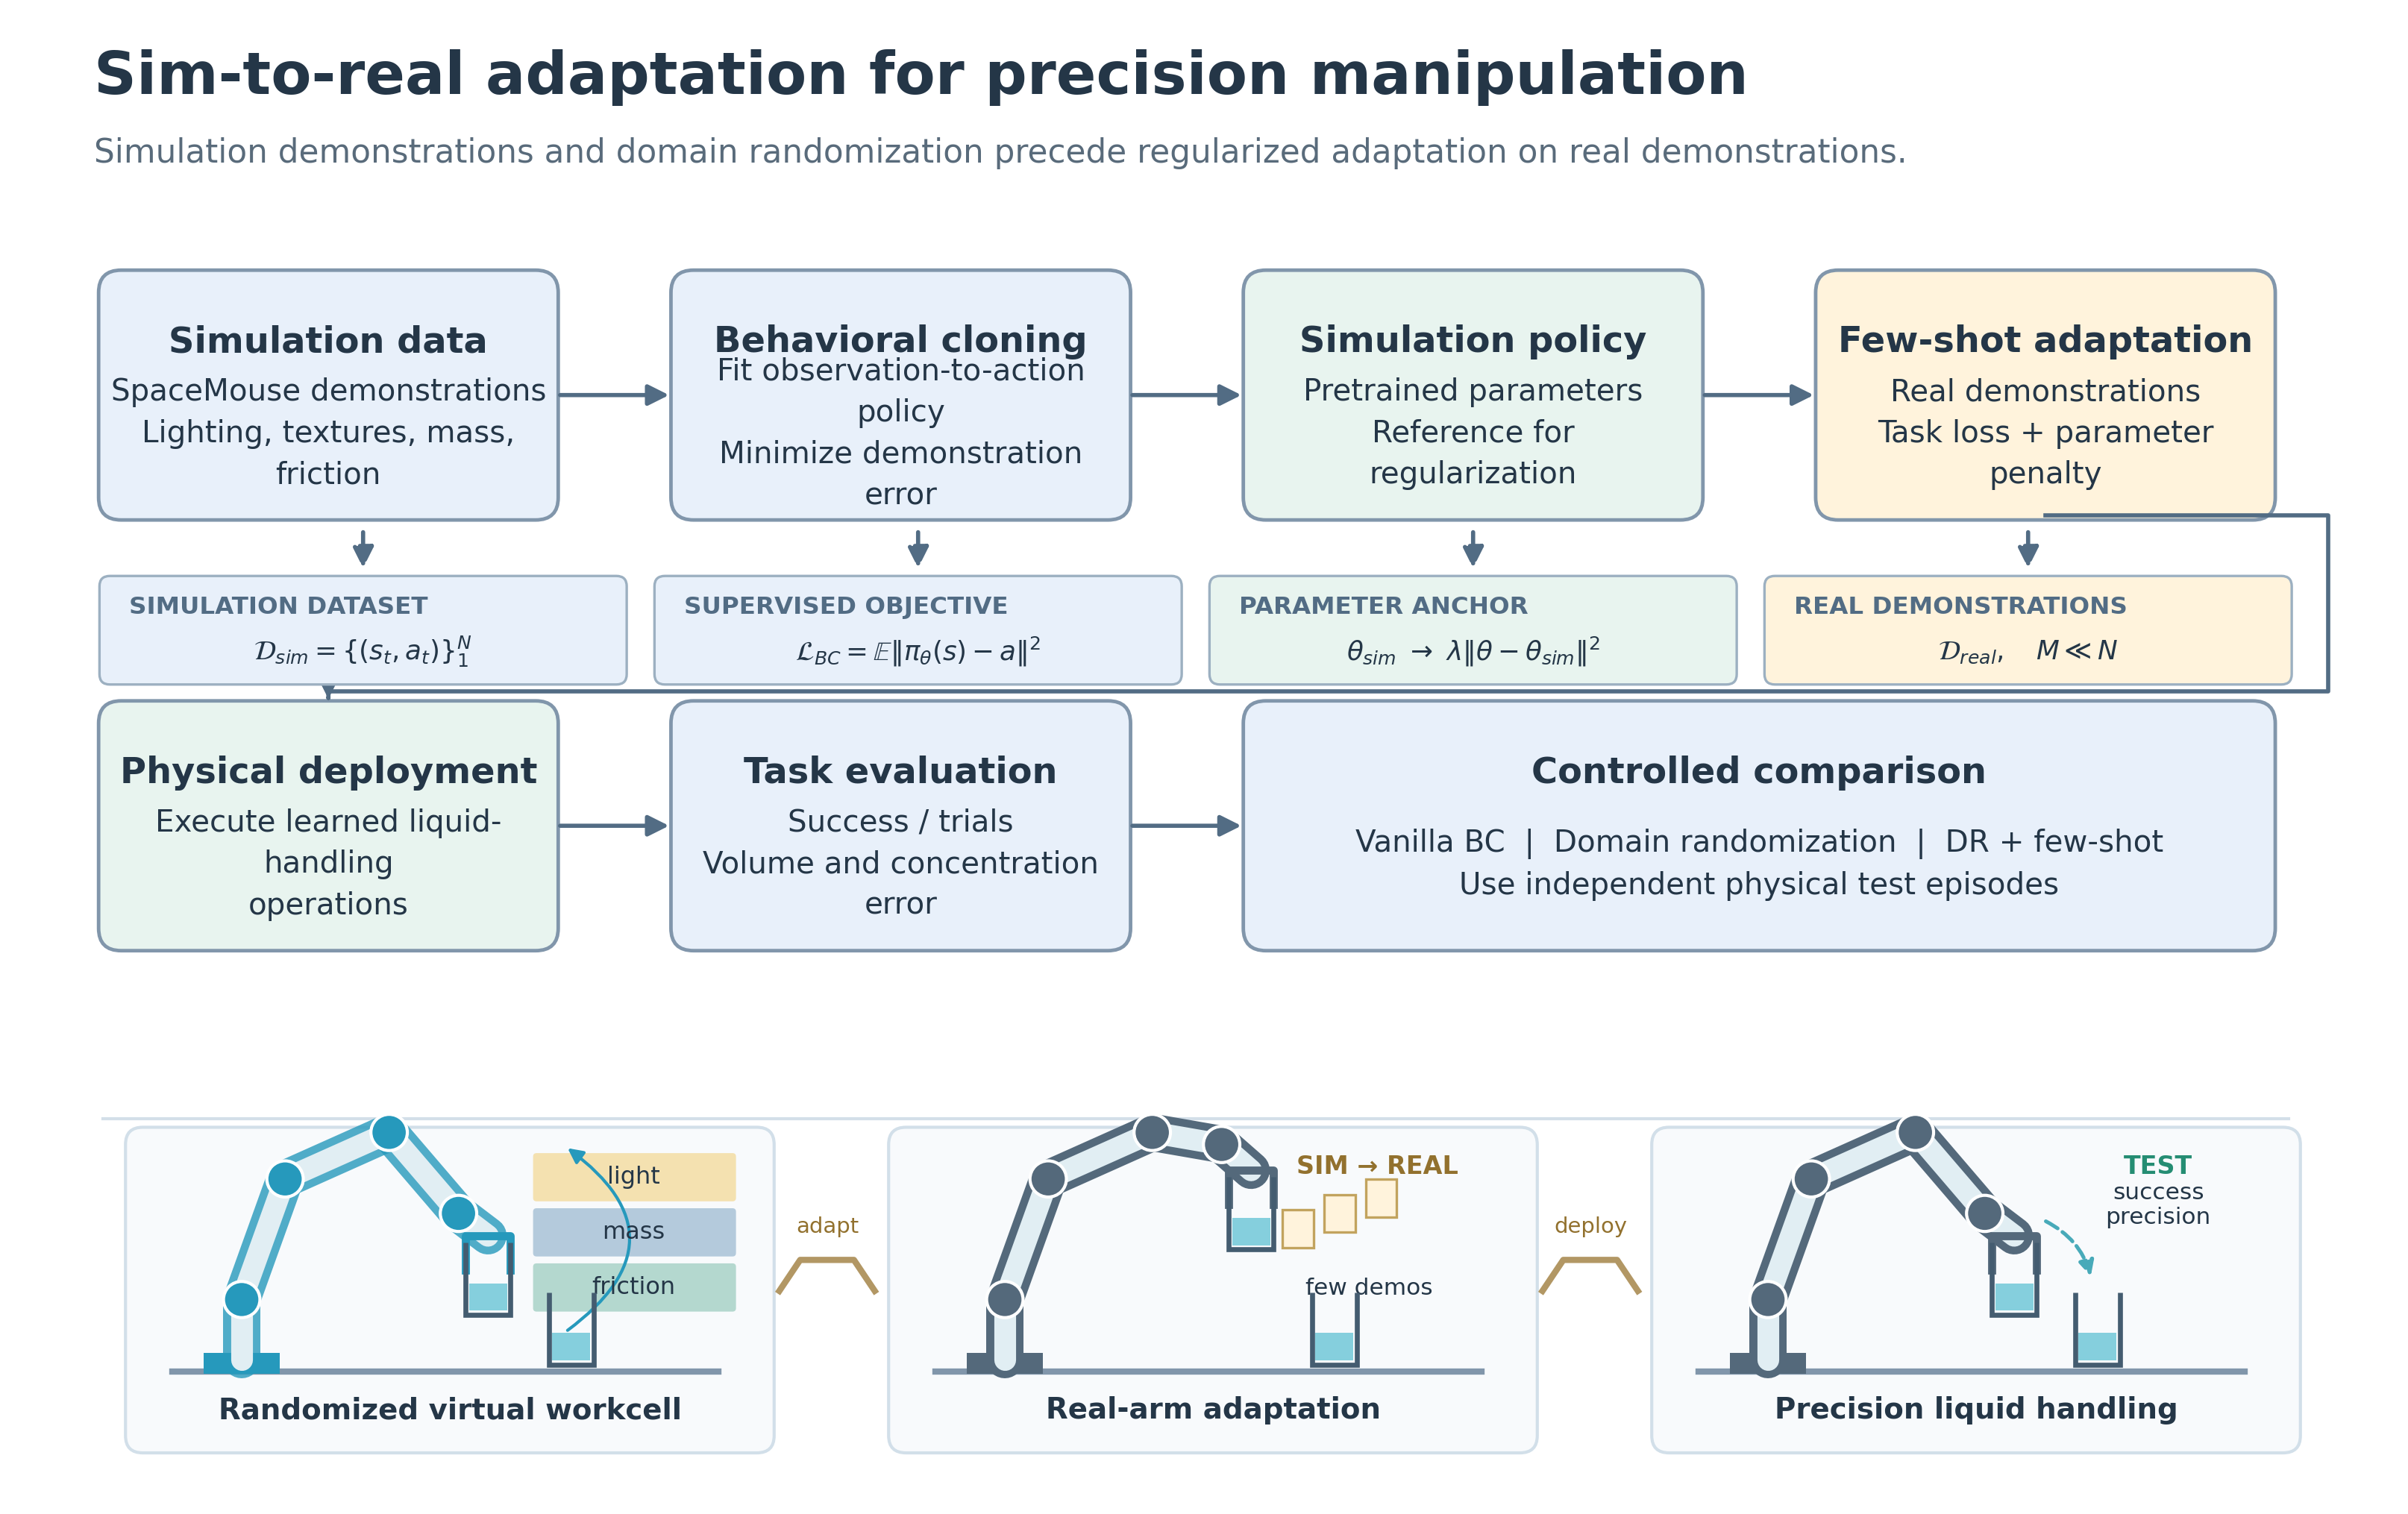
\includegraphics[width=\textwidth]{images/mechanisms/sim_to_real_mechanism.png}
    \caption{精密操作的虚实迁移机制。行为克隆与域随机化提供仿真策略，少量实体示教用于带参数正则化的微调。桥梁示意适配与部署，对比模块表示评估方案而非额外训练步骤。机械臂为示意绘制。}
    \label{fig:sim_to_real_mechanism}
\end{figure*}

对于微量移液和液滴滴加等精度要求极高的微观操作，我们引入了遥操作引导的模仿学习（IL）管线。利用6自由度SpaceMouse接口在仿真中采集专家示教数据$\mathcal{D}_{\text{sim}} = \{(s_t, a_t)\}_{i=1}^N$，并通过行为克隆（BC）预训练视觉运动策略$\pi_\theta(a_t | s_t)$：
\begin{equation}
    \mathcal{L}_{\text{BC}}(\theta) = \mathbb{E}_{(s_t, a_t) \sim \mathcal{D}_{\text{sim}}} \left[ \left\| \pi_\theta(s_t) - a_t \right\|_2^2 \right]
\end{equation}
仿真训练期间应用了包含光照、纹理、物体质量和摩擦系数的域随机化（DR）。

为了弥合由液体表面张力、光学折射和夹爪柔顺形变引起的真实世界虚实鸿沟，我们利用极少量（$M$组）物理示教实施了带正则化的少样本真实世界微调机制。策略参数通过最小化以下目标自适应调整为$\theta_{\text{real}}$：
\begin{equation}
    \theta_{\text{real}} = \arg\min_{\theta} \left( \mathbb{E}_{(s_t, a_t) \sim \mathcal{D}_{\text{real}}} \left[ \left\| \pi_\theta(s_t) - a_t \right\|_2^2 \right] + \lambda \left\| \theta - \theta_{\text{sim}} \right\|_2^2 \right)
\end{equation}
其中$\lambda$为正则化超参数，防止对仿真学到特征的灾难性遗忘，实现了鲁棒的物理部署。

为了缓解行为克隆固有的分布偏移问题，我们还采用了DAgger（数据集聚合）方法，该方法在学习者自身的状态分布下迭代采集纠正示教：
\begin{equation}
    \mathcal{D}_{\text{DAgger}} = \mathcal{D}_{\text{sim}} \cup \left\{ \left( s_t^{\pi_\theta}, \, a_t^{\text{expert}} \right) \right\}_{t=1}^{T}
\end{equation}
其中$s_t^{\pi_\theta}$为当前策略访问的状态，$a_t^{\text{expert}}$为专家纠正动作。聚合数据集用于重新训练策略，逐步减少复合误差。

此外，对于需要多模态动作分布的任务，我们引入了受GAIL \cite{ho2016gail}启发的基于判别器的对抗损失：
\begin{equation}
    \min_{\theta} \max_{\omega} \; \mathbb{E}_{\pi_\theta} \left[ \log D_\omega(s, a) \right] + \mathbb{E}_{\mathcal{D}_{\text{expert}}} \left[ \log(1 - D_\omega(s, a)) \right] - \lambda_{\text{ent}} \mathcal{H}[\pi_\theta]
\end{equation}
其中$D_\omega$为学习到的判别器，用于区分专家生成和策略生成的状态转移，$\lambda_{\text{ent}}$为熵奖励系数。

\subsection{具备失败恢复机制的分层状态机与技能库}
\label{subsec:hierarchical_skill}

图~\ref{fig:hsm_recovery_mechanism}展示基于条件的技能编排，以及验证失败后的有限次数恢复。
\begin{figure*}[!t]
    \centering
    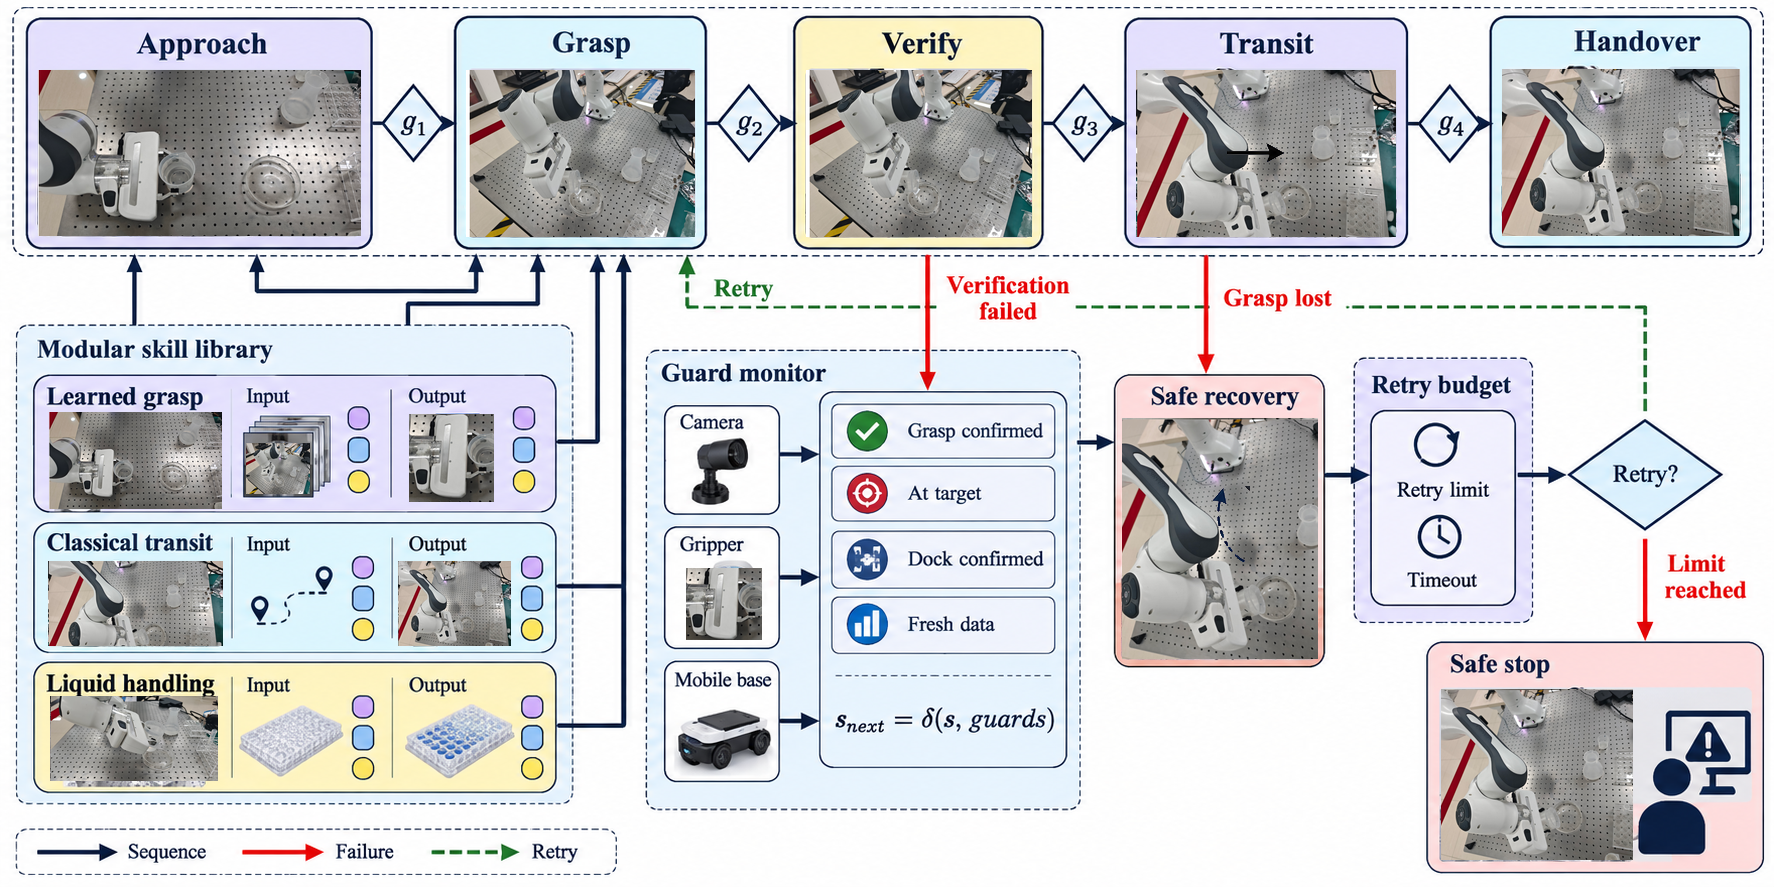
\includegraphics[width=\textwidth]{images/mechanisms/hsm_recovery_reference_style_panda_photos.png}
    \caption{具备失败恢复机制的分层状态机与模块化技能库。完成条件允许顺序推进，验证失败或抓取丢失触发有限安全恢复，达到重试或超时上限则安全停止。Panda画面直接裁剪自原始实验照片并复用于设备示意，不是交接或恢复阶段的独立实验证据；其余图标为示意，不表示经训练的高层策略或已测得的恢复收益。}
    \label{fig:hsm_recovery_mechanism}
\end{figure*}

为协调抓取、转移和移液等多阶段任务，我们在模块化\textit{技能库}之上采用规则驱动的分层状态机（HSM）。上层任务编排不是经训练的强化学习策略；其作用是将任务顺序、状态转移和失败恢复条件显式定义。

技能库$\mathcal{L}_{\text{skills}} = \{\pi_{\text{grasp}}, \pi_{\text{transit}}, \pi_{\text{pour}}, \dots\}$包含独立实现的操作策略及经典规划程序。每个技能规定前置条件、完成判据、超时限制和失败代码。模块化允许单独更新某一技能，但若无与单体策略的对照实验，不能宣称已消除负迁移。

状态机包含\texttt{approach}、\texttt{grasp}、\texttt{verify}、\texttt{transit}、\texttt{handover}和\texttt{recover}等状态。预定义条件检查\texttt{is\_bottle\_grasped}、\texttt{is\_at\_target}、对接确认和传感器数据新鲜度。给定当前状态与条件结果，转移$s_{t+1}=\delta(s_t,g(o_t))$是确定性的；本文不假设状态转移概率或学习得到的置信度。


若抓取验证失败，状态机停止转移，并在安全重新定位后返回\texttt{grasp}。重试次数与超时限制约束重复尝试；达到上限则进入安全停止状态，等待人工检查。这是所定义的恢复机制，不等于已经证实恢复率提升。应与无恢复机制的固定顺序状态机比较，报告阶段及完整工作流成功率、恢复次数、人工干预次数和完成时间。
